% ----------------------------------------------------------
% Introdução
% ----------------------------------------------------------
\chapter{Introdução}
\label{cap:introducao}
% ----------------------------------------------------------

No mundo contemporâneo, marcado pela conectividade e pelos avanços tecnológicos, a cultura e as artes encontram na tecnologia uma aliada poderosa para sua promoção e difusão. A Casa de Cultura de Monlevade, desempenhando o importante papel de Secretaria Municipal de Cultura na cidade de João Monlevade, tem buscado formas inovadoras de fomentar o talento artístico local. Nesse contexto, o desenvolvimento de uma plataforma de artistas monlevadenses surge como uma iniciativa que visa valorizar e promover a riqueza cultural da região.

No entanto, a criação de uma plataforma cultural esbarra em um desafio recorrente enfrentado por muitas iniciativas culturais no Brasil: a escassez de recursos financeiros. Em um cenário de cortes orçamentários e falta de investimentos, torna-se ainda mais desafiador obter os recursos necessários para viabilizar projetos como esse. É nesse contexto que se busca por alternativas criativas e parcerias gratuitas para tornar possível a concretização da plataforma de artistas monlevadenses.

% ----------------------------

\section{Elaboração do capítulo}

Este capítulo apresenta o seu trabalho. Você deve contextualizar o problema abordado, descrever os objetivos gerais e específicos, apresentar a metodologia e como o trabalho está estruturado.

\section{O problema de pesquisa}
\label{sec:problema}

O desenvolvimento de uma plataforma de artistas monlevadenses para a Casa de Cultura esbarra na dificuldade em obter recursos financeiros para sua realização. Em um contexto de restrições orçamentárias e escassez de investimentos na cultura, torna-se desafiador viabilizar a criação de uma plataforma digital que promova a cultura local e valorize os talentos artísticos de Monlevade. A falta de recursos financeiros adequados e sustentáveis se apresenta como um obstáculo para o desenvolvimento e a manutenção dessa iniciativa cultural, comprometendo seu potencial de impacto e alcance na comunidade.

Compreender os desafios relacionados à captação de recursos e buscar alternativas viáveis para financiar o projeto é fundamental para tornar possível a implementação e a continuidade da plataforma de artistas monlevadenses. É necessário encontrar estratégias e parcerias que permitam superar as restrições orçamentárias e garantir a sustentabilidade financeira dessa plataforma, a fim de fortalecer a cultura local, promover a divulgação das obras de arte e proporcionar uma experiência enriquecedora para o público.

Assim, o problema de pesquisa deste trabalho consiste em como superar a dificuldade em obter recursos financeiros para o desenvolvimento da plataforma de artistas monlevadenses, buscando estratégias de captação de recursos e parcerias que permitam sua viabilização e sustentabilidade financeira, garantindo o acesso à cultura e valorizando os talentos artísticos presentes em Monlevade.

\subsection{Introdução à Casa de Cultura de João Monlevade}
%Confirmar dados com a casa de cultura 
A Casa de Cultura de João Monlevade desempenha um papel importante no desenvolvimento social e na promoção da cultura local. A instituição foi fundada em 1948 por uma iniciativa de um grupo de intelectuais e artistas locais que perceberam a necessidade de um local dedicado à apreciação das expressões culturais monlevadenses. A Casa de Cultura tem sido um local onde as pessoas se reúnem e celebram a cultura desde então, e ela desempenha um papel importante na vida cultural da cidade.

Ao longo dos anos, a Casa de Cultura tem se destacado por sua diversidade de atividades e qualidade. Apresentações musicais, escola de artes,oficinas, dança e literatura estão entre as atividades da instituição. Além de promover a cultura local, essas atividades visam incentivar a produção artística e intelectual da região, promovendo o debate cultural na comunidade.

A Casa de Cultura tem um público diversificado, desde crianças até idosos. Eles sempre estão procurando oferecer programações e atividades que atendam às diferentes faixas etárias e interesses. Além disso, a organização mantém fortes vínculos com as escolas e com os grupos comunitários, promovendo de forma integrada a educação e a cultura.

O significado da Casa de Cultura de João Monlevade vai além da área cultural. A organização ajuda a construir uma consciência histórica e cultural entre os habitantes locais, promovendo a identidade e a memória da cidade. Além disso, a Casa de Cultura contribui para o enriquecimento da vida cultural da cidade, desempenhando um papel importante na formação de novos talentos e na promoção da diversidade cultural.

Atualmente, a Casa de Cultura de João Monlevade está presente em diversas redes sociais, como por exemplo o Instagram e o Facebook. Através de suas páginas nessas redes, os funcionários da Casa de Cultura publicam sobre eventos próximos e futuros organizados por eles, além de divulgar vagas para os cursos da escola de artes, presente dentro da sede. Essa interação mais próxima com a população se tornou cada vez mais importante, tendo em vista a facilidade de comunicação com o publico alvo através dessas ferramentas.

Assim, a Casa de Cultura de João Monlevade é algo mais do que apenas um promotor de eventos culturais. É um símbolo da identidade e da história da cidade, e também um centro de irradiação cultural que melhora a vida dos habitantes e promove a inclusão social por meio da cultura. Seus esforços para preservar e promover a cultura local são inestimáveis, tornando-a um patrimônio cultural e social significativamente valioso para a comunidade monlevadense.


\subsection{A relevância da internet e dos sites web para a cultura}
Nos dias atuais, não há dúvida de quão importantes são a internet e os sites web para a cultura. Com o uso crescente da internet como meio de comunicação e divulgação cultural, as organizações culturais têm encontrado uma maneira eficaz de atingir um público cada vez mais amplo e diversificado.

Uma das principais vantagens de ter um site web para uma instituição cultural é aumentar sua visibilidade e alcance. Atualmente, sem um grande investimento em publicidade e marketing, uma instituição cultural não poderia alcançar apenas o público local, mas também aqueles de outras regiões e até mesmo de outros países.

Além disso, o público interessado pode acessar informações por meio de um site. Ele pode fornecer informações sobre a história, missão, projetos e atividades da instituição. Ele também pode fornecer informações práticas, como horários de funcionamento, formas de contato e rotas para chegar lá. Isso facilita a interação do público com a instituição e sua participação em suas atividades.

A capacidade de promover eventos e atividades culturais de forma mais eficaz é outra vantagem de ter um site web. Ao divulgar programações, exposições, espetáculos, cursos e workshops no site, é possível alcançar um público maior e garantir que mais pessoas participem das atividades da instituição. Um site online ajuda a fortalecer a cultura da comunidade, aumenta o envolvimento e o orgulho dos habitantes locais ao fornecer informações sobre a cultura local, sua história, tradições e artistas.

Como resultado, a internet e os sites web são hoje uma ferramenta vital para as instituições culturais, permitindo não apenas um maior alcance e visibilidade, mas também uma maior interação e participação do público. Uma instituição cultural desenvolvendo um site web está contribuindo para a promoção da cultura e o fortalecimento da identidade cultural da comunidade.

A digitalização da cultura e a presença online das instituições culturais também permitem a preservação e disseminação do patrimônio cultural de maneira inédita. Arquivos digitais, galerias de imagens, vídeos de performances e gravações de áudio podem ser disponibilizados online, garantindo que um público global tenha acesso a esses recursos. Essa disponibilidade perpetua o conhecimento cultural, tornando-o acessível para futuras gerações, independentemente das barreiras geográficas.

Além da disseminação de informações, os sites web oferecem um espaço para a experimentação e inovação cultural. Plataformas online podem ser utilizadas para criar exposições virtuais, apresentações interativas e outras formas de arte digital. Esses novos formatos não apenas expandem as possibilidades de expressão artística, mas também atraem públicos que talvez não frequentem eventos culturais tradicionais. Dessa forma, a internet se torna um campo fértil para a criação e a reinvenção cultural.

Outro aspecto importante é o papel dos sites web na educação cultural. Instituições culturais podem oferecer cursos online, workshops e palestras, acessíveis a qualquer pessoa com conexão à internet. Esse tipo de oferta educativa amplia o impacto social das instituições culturais, permitindo que mais pessoas tenham acesso a conhecimentos especializados e a oportunidades de desenvolvimento pessoal e profissional.

Finalmente, os sites web permitem uma comunicação bidirecional entre as instituições culturais e seu público. Por meio de comentários, fóruns e redes sociais integradas, os usuários podem interagir diretamente com as instituições, expressar suas opiniões e participar de discussões sobre temas culturais. Essa interação promove um senso de comunidade e pertencimento, além de proporcionar às instituições um feedback valioso para melhorar suas ofertas e serviços.

Em conclusão, a internet e os sites web transformaram a maneira como a cultura é compartilhada, promovida e consumida. Eles oferecem inúmeras vantagens para as instituições culturais, desde o aumento da visibilidade e alcance até a preservação do patrimônio cultural e a inovação artística. Ao desenvolver uma presença online robusta, as instituições culturais não apenas ampliam seu impacto, mas também fortalecem a identidade cultural e a coesão social das comunidades que servem.

\subsection{Tecnologias para desenvolvimento de sites web}

As principais tecnologias utilizadas para o desenvolvimento web são bem conhecidas. A um nível básico e falando de forma análoga, primeiramente temos o HTML, que seria uma folha de papel onde podemos estruturar nosso site. Para deixa-lo com a nossa cara, modificamos seu CSS, como se estivéssemos colorindo essa folha de papel. E caso seja necessário que essa folha de papel tenha alguma animação, ou uma automação de algum tipo, usamos o JavaScript para dar vida a pagina.

Apesar de ser posivel fazer varias paginas usando somente essas 3 tecnologias, em algum momento ficara faltando algo ou seria muito trabalhoso desenvolver tudo do zero. Com esse problema, desenvolvedores criaram frameworks e bibliotecas para facilitar e agilizar o desenvolvimento web. Dentre eles temos o React, uma biblioteca JavaScript para a construção de interfaces de usuário, especialmente de aplicativos de página única (SPAs) e o Angular, outro framework JavaScript desenvolvido pelo Google para a construção de aplicativos web dinâmicos.

Quando se precisa de um framework ainda mais robusto, que auxilie na criacao de sites no estilo blog, ou que armazenaram dados, noticias ou outras coisas similares, pode-se utilizar sistemas Gerenciadores de Conteúdo (CMS). Esses sistemas facilitam ainda mais a criacao e manutencao de sites com varias funcionalidades, ajudando na utilizacao de banco de dados, criacao de conteudo e ate mesmo na otimizacao para ferramentas de pesquisa (SEO). Dentre os principais atualmente temos o Wordpress, o CMS mais popular, usado para criar e gerenciar sites e blogs com facilidade. Ele oferece uma vasta gama de plugins e temas, facilitando a personalização e a adição de funcionalidades ao site. O Joomla e um CMS de código aberto que permite a criação de sites poderosos e complexos que oferece flexibilidade e uma comunidade ativa, tornando-o uma escolha robusta para sites de médio a grande porte. O Drupal, um CMS altamente flexível e escalável, ideal para sites que requerem uma personalização intensa, esse e conhecido por sua segurança e capacidade de gerenciar grandes volumes de conteúdo.

Assim viu-se indispensável a utilização de um sistema CMS. Para definir qual das tecnologias seria mais adequada, necessita-se atenção a quais serão as funcionalidades desse sistema e qual objetivo ele quer cumprir. Tendo em vista que o site para a Casa de Cultura de João Monlevade teria dois objetivos principais, sendo esses servir como meio para divulgar noticias e editais da Casa de Cultura e ser também um sistema de gestão para a escola de artes, procurou-se um CMS que possibilitasse essa multitarefa.

O CodeRed CMS é um sistema de gerenciamento de conteúdo baseado no framework Django e no CMS Wagtail. Ele foi projetado para facilitar a criação e a gestão de sites empresariais, com foco em flexibilidade, desempenho e facilidade de uso. o Django é um dos frameworks mais robustos e escaláveis para desenvolvimento web, conhecido por sua segurança e capacidade de lidar com grandes volumes de dados e tráfego. Já o Wagtail e Um CMS flexível e poderoso, desenvolvido sobre o Django, que oferece uma interface de administração amigável e recursos avançados de gestão de conteúdo.

Esse sistema possui funcionalidades avançadas para a gestão de conteúdo. A flexibilidade na criação de páginas, permite a criação de páginas personalizadas com componentes reutilizáveis, facilitando a construção de layouts complexos sem a necessidade de códigos complexos ou repetitivos. Auxilia na publicação de notícias e editais, oferecendo ferramentas integradas para a publicação e gerenciamento de conteúdos como notícias e editais, com recursos de agendamento e controle de versões.

Além de uma interface amigável para a criação de novos conteúdos como artigos e editais, o sistema possibilita a utilização de outra interface que poderá ser acessada por administradores do sistema, o django-admin. Esta vem por padrão quando se utiliza o Django e oferece facilidade na modificação de informações, além de acesso direto aos dados guardadas no banco de dados do site, o que será importante para as funcionalidades da Escola de Artes.

A capacidade de integração do CodeRed CMS com outras ferramentas e sistemas também é um fator crucial para sua escolha. A Casa de Cultura de João Monlevade, ao utilizar esse CMS, poderá facilmente incorporar sistemas de pagamento, plataformas de e-mail marketing e outras aplicações essenciais para o gerenciamento das suas atividades culturais e educacionais. Essa integração garante que todas as necessidades operacionais e administrativas possam ser centralizadas em um único sistema, aumentando a eficiência e a eficácia da gestão.

Outra vantagem significativa do CodeRed CMS é a sua robusta estrutura de segurança. Desenvolvido sobre o Django, que é conhecido por suas práticas de segurança integradas, o sistema oferece proteção contra ataques comuns, como SQL injection, cross-site scripting (XSS) e cross-site request forgery (CSRF). Isso é particularmente importante para a Casa de Cultura de João Monlevade, que pode lidar com dados sensíveis dos usuários e transações financeiras.

A escalabilidade do CodeRed CMS também é um ponto forte. Conforme a Casa de Cultura de João Monlevade cresce e expande suas atividades, o CMS pode acompanhar esse crescimento sem comprometer o desempenho. O Django, com seu suporte a grandes volumes de dados e tráfego, assegura que o site permanecerá rápido e responsivo, mesmo com um aumento significativo no número de visitantes e conteúdos publicados.

A facilidade de uso do Wagtail, que é a base do CodeRed CMS, proporciona uma experiência administrativa intuitiva. A interface de arrastar e soltar, juntamente com a capacidade de pré-visualizar as alterações antes de publicá-las, facilita o trabalho dos administradores do site, que podem não ter habilidades técnicas avançadas. Isso permite que a equipe da Casa de Cultura de João Monlevade se concentre mais na criação e gestão de conteúdo de qualidade, ao invés de se preocupar com os aspectos técnicos da manutenção do site.

Além disso, o CodeRed CMS suporta práticas de SEO avançadas, essenciais para aumentar a visibilidade online da Casa de Cultura de João Monlevade. Ferramentas integradas ajudam a otimizar o conteúdo para motores de busca, melhorando o ranking do site nos resultados de pesquisa e atraindo mais visitantes. Com uma estratégia de SEO bem implementada, a Casa de Cultura pode alcançar um público mais amplo, promovendo suas atividades e eventos de maneira mais eficaz.

A escolha do CodeRed CMS também se justifica pela possibilidade de personalização e extensão das suas funcionalidades. A Casa de Cultura de João Monlevade pode, por exemplo, desenvolver módulos específicos para atender a necessidades particulares, como a gestão de inscrições para cursos e workshops, acompanhamento de presença dos alunos, e avaliação de performances artísticas. Essa capacidade de personalização garante que o sistema possa evoluir junto com as demandas específicas da instituição.

A manutenção e atualização do site também são facilitadas pelo uso do CodeRed CMS. A comunidade ativa de desenvolvedores de Django e Wagtail oferece suporte contínuo, documentação extensa e atualizações regulares, o que garante que o sistema esteja sempre atualizado com as últimas inovações tecnológicas e práticas de segurança. Isso reduz o risco de vulnerabilidades e garante que o site opere de maneira eficiente e segura.

Outro aspecto importante é a capacidade do CodeRed CMS de fornecer análises detalhadas sobre o comportamento dos usuários. Integrado com ferramentas de análise como Google Analytics, o sistema permite que a Casa de Cultura de João Monlevade monitore o tráfego do site, entenda as preferências dos visitantes e tome decisões informadas sobre o conteúdo e as funcionalidades a serem aprimoradas. Esse conhecimento detalhado do público-alvo é crucial para a criação de estratégias de engajamento mais eficazes e para a otimização da experiência do usuário.

Além disso, a integração do CodeRed CMS com plataformas de mídias sociais facilita a promoção das atividades da Casa de Cultura. Compartilhar eventos, exposições e outras atividades diretamente nas redes sociais ajuda a aumentar a visibilidade e a atrair um público maior. As funcionalidades de compartilhamento social integradas garantem que os conteúdos possam ser facilmente divulgados, aumentando o alcance e o impacto das campanhas de marketing digital.

A utilização do CodeRed CMS também contribui para a sustentabilidade da Casa de Cultura de João Monlevade. Um sistema eficiente de gerenciamento de conteúdo reduz a necessidade de recursos físicos, como papel para folhetos e cartazes, substituindo-os por versões digitais acessíveis online. Isso não apenas diminui os custos operacionais, mas também apoia práticas ambientalmente responsáveis.

A interface do usuário do Wagtail, intuitiva e amigável, facilita a capacitação da equipe da Casa de Cultura. Com um treinamento básico, os administradores do site podem rapidamente aprender a criar, editar e publicar conteúdos, garantindo que a plataforma seja utilizada de maneira eficiente. A facilidade de uso incentiva a equipe a atualizar regularmente o site, mantendo-o sempre relevante e atualizado para os visitantes.

Em termos de design, o CodeRed CMS permite a implementação de um site visualmente atraente e alinhado com a identidade visual da Casa de Cultura de João Monlevade. A flexibilidade na personalização do layout e a disponibilidade de templates pré-desenvolvidos proporcionam um design profissional sem a necessidade de investimentos significativos em desenvolvimento gráfico. Isso é fundamental para transmitir a imagem e os valores da instituição de maneira coerente e atraente.

Por fim, o suporte a múltiplos idiomas é uma funcionalidade relevante do CodeRed CMS. Considerando a diversidade cultural e o potencial interesse de visitantes internacionais, a possibilidade de oferecer conteúdo em diferentes idiomas amplia o alcance do site e facilita o acesso de um público global. Essa funcionalidade é particularmente importante para a promoção de eventos e exposições que possam atrair turistas e estudiosos de outros países.

Em conclusão, a escolha do CodeRed CMS para o desenvolvimento do site da Casa de Cultura de João Monlevade é fundamentada em uma série de benefícios que incluem flexibilidade, segurança, escalabilidade, facilidade de uso, capacidade de personalização e suporte a práticas de SEO e marketing digital. Essas características garantem que o site não apenas atenda às necessidades imediatas da instituição, mas também esteja preparado para evoluir e crescer junto com ela, promovendo a cultura e o desenvolvimento social da comunidade de maneira eficaz e sustentável.

\subsection{Usabilidade e acessibilidade de sites web}

A usabilidade e a acessibilidade são elementos cruciais para garantir que um site seja fácil de usar e acessível a todos os públicos, incluindo pessoas com deficiência. A usabilidade refere-se à eficiência, eficácia e satisfação com que os usuários podem realizar tarefas em um site, enquanto a acessibilidade diz respeito à capacidade do site de ser utilizado por pessoas com diversas deficiências. Para criar um site verdadeiramente inclusivo, é essencial seguir diretrizes e princípios que promovam tanto a usabilidade quanto a acessibilidade.

Primeiramente, a simplicidade e clareza da interface são fundamentais para a usabilidade. Uma interface bem projetada deve ser intuitiva e fácil de entender, mesmo para usuários que a estão acessando pela primeira vez. Isso inclui a organização lógica dos elementos, a utilização de uma linguagem clara e a minimização da complexidade. A adoção de uma abordagem minimalista, onde apenas os elementos essenciais são destacados, pode ajudar a evitar a sobrecarga de informações e tornar a navegação mais fluida.

Além da simplicidade, a navegação intuitiva é um aspecto vital para a usabilidade. Os menus e as opções de navegação devem ser organizados de forma coerente, permitindo que os usuários encontrem facilmente o que procuram. Elementos de navegação como barras de menu, botões e links devem ser visíveis e consistentes em todas as páginas do site. Adotar padrões conhecidos e evitar mudanças drásticas na estrutura de navegação pode melhorar significativamente a experiência do usuário.

A acessibilidade vai além da usabilidade, garantindo que o conteúdo do site esteja disponível e utilizável por pessoas com deficiências visuais, auditivas e motoras. Para alcançar esse objetivo, é necessário seguir diretrizes específicas, como as estabelecidas pela Web Content Accessibility Guidelines (WCAG). Essas diretrizes fornecem recomendações detalhadas para tornar o conteúdo web mais acessível.

Para pessoas com deficiências visuais, é importante que o site seja compatível com leitores de tela. Isso inclui o uso adequado de tags alt para descrever imagens, a estruturação correta do HTML para que os leitores de tela possam interpretar a página de maneira lógica e a garantia de contraste adequado entre o texto e o fundo para facilitar a leitura. Além disso, oferecer opções de aumentar o tamanho da fonte pode ser benéfico para usuários com baixa visão.

Para tornar o conteúdo acessível a pessoas com deficiências auditivas, é essencial fornecer alternativas textuais para qualquer conteúdo de áudio ou vídeo. Legendas, transcrições e descrições de áudio são recursos importantes que garantem que essas informações possam ser acessadas por todos. Em vídeos, as legendas sincronizadas e as transcrições ajudam a transmitir a mensagem de maneira eficaz.

A acessibilidade para pessoas com deficiências motoras pode ser melhorada garantindo que o site possa ser navegado usando apenas o teclado, sem a necessidade de um mouse. Os elementos clicáveis devem ser suficientemente grandes e espaçados para facilitar o uso por pessoas com mobilidade limitada. Além disso, implementar atalhos de teclado pode acelerar a navegação para usuários que dependem desses dispositivos.

Para garantir que a Casa de Cultura de João Monlevade ofereça um site inclusivo, é vital incorporar as melhores práticas de usabilidade e acessibilidade desde o início do processo de desenvolvimento. Uma abordagem proativa à acessibilidade não apenas beneficia os usuários com deficiências, mas também melhora a experiência geral para todos os visitantes do site.

Um dos primeiros passos para alcançar uma boa acessibilidade é realizar testes com usuários reais, incluindo pessoas com diferentes tipos de deficiência. Esses testes fornecem insights valiosos sobre os desafios que esses usuários enfrentam e ajudam a identificar áreas de melhoria que podem não ser evidentes para desenvolvedores sem essas experiências. Feedback direto dos usuários é uma ferramenta poderosa para refinar a usabilidade e garantir que as soluções implementadas realmente atendam às suas necessidades.

Além disso, a implementação de padrões e ferramentas de acessibilidade deve ser uma prática contínua. Ferramentas como validadores de acessibilidade e verificadores de contraste de cores podem ajudar a identificar e corrigir problemas de acessibilidade durante o desenvolvimento. Manter-se atualizado com as diretrizes WCAG e outras normas de acessibilidade garante que o site continue a ser acessível à medida que novas tecnologias e padrões emergem.

O treinamento da equipe da Casa de Cultura de João Monlevade em princípios de usabilidade e acessibilidade é igualmente importante. Capacitar os administradores e criadores de conteúdo para entender e aplicar essas práticas assegura que o site permaneça acessível a longo prazo. Treinamentos regulares e recursos educacionais sobre acessibilidade web podem ajudar a manter a equipe informada sobre as melhores práticas e novos desenvolvimentos na área.

Além dos aspectos técnicos, a acessibilidade também envolve considerar as necessidades culturais e linguísticas dos usuários. Para uma instituição cultural como a Casa de Cultura de João Monlevade, é essencial que o site reflita a diversidade e a riqueza cultural da comunidade. Oferecer conteúdo em múltiplos idiomas e garantir que as traduções sejam precisas e culturalmente relevantes é uma forma de tornar o site mais inclusivo e acessível para um público mais amplo.

Outro elemento crucial é a personalização da experiência do usuário. Permitir que os visitantes ajustem as configurações do site de acordo com suas preferências individuais, como tamanhos de fonte, esquemas de cores e opções de contraste, pode melhorar significativamente a usabilidade e a acessibilidade. Funcionalidades como modos de alto contraste e leitores de texto integrados são exemplos de como a personalização pode atender a diversas necessidades de acessibilidade.

Para promover a inclusão digital, é importante também considerar a acessibilidade em dispositivos móveis. Com o crescente uso de smartphones e tablets para acessar a internet, o site da Casa de Cultura de João Monlevade deve ser responsivo e oferecer uma experiência de usuário consistente em todas as plataformas. Garantir que o design seja mobile-first, ou seja, otimizado primeiro para dispositivos móveis e depois adaptado para desktops, pode ser uma estratégia eficaz para alcançar essa meta.

Assim, é essencial que a acessibilidade e a usabilidade sejam vistas como uma responsabilidade contínua e colaborativa. Manter um diálogo aberto com a comunidade de usuários, incluindo aqueles com deficiências, e estar disposto a adaptar e melhorar o site com base em suas necessidades e feedbacks, é a chave para criar um ambiente digital verdadeiramente inclusivo. A construção do site, ao adotar uma abordagem centrada no usuário para a acessibilidade, não apenas cumpre suas obrigações legais e éticas, mas também reforça seu compromisso com a inclusão e a equidade.


\subsection{Segurança da informação em sites web}

A proteção da informação em sites da web é uma questão crucial, especialmente para instituições como a Casa de Cultura de João Monlevade, que lida com dados sensíveis de usuários e informações essenciais para suas atividades. Os principais desafios em termos de segurança incluem as ameaças de hackers, malware e phishing, todos capazes de causar danos significativos, desde a interrupção dos serviços até o comprometimento dos dados pessoais dos usuários.

Os ataques cibernéticos representam uma das maiores ameaças à segurança dos sites da web. Esses ataques podem se manifestar de várias formas, incluindo invasões para roubo de informações, defacement (alteração maliciosa do conteúdo do site) e ataques de negação de serviço (DDoS), que podem tornar o site inacessível aos usuários. Para mitigar esses riscos, é vital adotar medidas robustas de segurança, como firewalls, sistemas de detecção de intrusos e a configuração adequada dos servidores.

Outra ameaça relevante é o malware, software malicioso criado para danificar, explorar ou desativar sistemas computacionais. O malware pode ser introduzido no site por diversas vias, incluindo downloads de arquivos infectados, vulnerabilidades em plugins e temas e até mesmo via anúncios maliciosos. Para manter o site seguro contra malwares, é fundamental manter o software sempre atualizado, fazer verificações de segurança frequentes e garantir que todos os plugins e temas sejam baixados de fontes confiáveis e atualizados regularmente.

O phishing é uma técnica de engenharia social usada para enganar os usuários e obter informações confidenciais, como nomes de usuário, senhas e detalhes de cartão de crédito. Sites fraudulentos que imitam o site legítimo da Casa de Cultura de João Monlevade podem ser usados para enganar os usuários. Para proteger contra phishing, é importante educar os usuários sobre os riscos e implementar medidas de autenticação robustas, como a autenticação de dois fatores (2FA).

Para garantir a segurança do site da Casa de Cultura de João Monlevade, a implementação de protocolos de segurança é essencial. Isso inclui o uso de HTTPS para criptografar a comunicação entre o navegador do usuário e o servidor, protegendo assim as informações transmitidas contra interceptação. Além disso, a implementação de certificados SSL/TLS é crucial para assegurar que os dados trocados permaneçam confidenciais e íntegros.

A atualização constante do software é outra medida crítica para a segurança do site. Manter o sistema operacional, servidores, CMS e todos os plugins e temas atualizados é vital para proteger contra vulnerabilidades conhecidas que podem ser exploradas por hackers. As atualizações de software frequentemente incluem patches de segurança que corrigem falhas recentemente descobertas, tornando o site mais seguro contra ataques.

A proteção contra ataques cibernéticos também envolve a realização de backups regulares dos dados do site. Ter backups atualizados garante que, em caso de um ataque bem-sucedido ou falha do sistema, o site possa ser restaurado rapidamente com a perda mínima de dados. Além disso, é recomendável implementar soluções de monitoramento e resposta a incidentes, que podem detectar atividades suspeitas e responder rapidamente para mitigar os danos.

Além das medidas mencionadas, é vital realizar auditorias regulares de segurança. Essas auditorias ajudam a identificar possíveis vulnerabilidades antes que sejam exploradas por atacantes. A realização de testes de penetração (pentests) é uma prática eficaz para avaliar a segurança do site, simulando ataques reais e identificando pontos fracos que necessitam de correção. A Casa de Cultura de João Monlevade deve considerar contratar profissionais de segurança cibernética para realizar essas avaliações periódicas.

A conscientização e o treinamento dos funcionários também desempenham um papel crucial na segurança da informação. Os funcionários devem ser treinados para reconhecer e responder a ameaças cibernéticas, como e-mails de phishing e outras tentativas de engenharia social. Programas de treinamento contínuo garantem que todos na organização estejam atualizados sobre as melhores práticas de segurança e saibam como proteger as informações sensíveis do site e dos usuários.

Outro aspecto importante é a gestão de acessos e permissões. O princípio do menor privilégio deve ser aplicado, garantindo que cada usuário tenha apenas o acesso necessário para realizar suas tarefas. Contas com privilégios administrativos devem ser limitadas e monitoradas rigorosamente para evitar abuso de acesso. Além disso, é importante desativar ou remover contas de usuários que não são mais necessárias para minimizar o risco de uso indevido.

A implementação de autenticação multifator (MFA) adiciona uma camada extra de segurança, exigindo que os usuários forneçam duas ou mais formas de verificação antes de acessar suas contas. Isso pode incluir algo que eles conhecem (como uma senha), algo que possuem (como um token ou smartphone) e algo que são (como biometria). A MFA reduz significativamente o risco de acesso não autorizado, mesmo que uma senha seja comprometida.

A política de gerenciamento de incidentes deve estar bem estabelecida. Isso inclui a definição de procedimentos claros para responder a incidentes de segurança, a comunicação interna e externa durante um incidente, e a recuperação e análise pós-incidente. Ter um plano de resposta a incidentes bem estruturado permite que a organização responda de maneira eficiente e minimize os impactos de quaisquer ataques cibernéticos.

Finalmente, a colaboração com outras organizações e a participação em comunidades de segurança cibernética pode fornecer insights valiosos e atualizações sobre as últimas ameaças e tendências de segurança. A troca de informações e melhores práticas com outras instituições culturais pode fortalecer as defesas cibernéticas da Casa de Cultura de João Monlevade.

A segurança da informação é uma preocupação contínua e multifacetada que requer uma abordagem proativa e abrangente. Para a Casa de Cultura de João Monlevade, a proteção dos dados e a manutenção da confiança dos usuários são essenciais para o sucesso de sua plataforma digital. Ao implementar medidas robustas de segurança, realizar auditorias regulares, treinar funcionários, gerenciar acessos de forma rigorosa e adotar tecnologias avançadas como a autenticação multifator, a instituição pode criar um ambiente seguro e confiável para todos os seus usuários.

Estas práticas não apenas protegem contra as ameaças cibernéticas, mas também garantem a continuidade das operações e a integridade das informações. A segurança deve ser vista como um componente essencial do desenvolvimento e manutenção do site, integrando-se a todas as fases do ciclo de vida do software. Através de um compromisso contínuo com a segurança da informação, a Casa de Cultura de João Monlevade pode cumprir sua missão de promover a cultura e servir a comunidade de maneira segura e eficiente.

\subsection{Trabalhos Relacionados}

A análise de trabalhos relacionados é fundamental para o desenvolvimento de um projeto de site para a Casa de Cultura de João Monlevade. Este capítulo aborda exemplos de sites web de Casas de Cultura no Brasil e no mundo, focando em suas funcionalidades, design e usabilidade, bem como na qualidade do conteúdo e informação disponibilizada. A identificação de boas práticas e tendências emergentes oferece uma base sólida para o desenvolvimento de um site que atenda às necessidades da comunidade e promova a cultura de maneira eficaz.

Para compreender melhor as melhores práticas na criação de sites para Casas de Cultura, foram analisados vários exemplos, tanto nacionais quanto internacionais. A seleção incluiu instituições com características semelhantes à Casa de Cultura de João Monlevade, permitindo uma comparação direta e a extração de elementos aplicáveis ao contexto local.

A Casa de Cultura Laura Alvim, localizada no Rio de Janeiro, possui um site que se destaca pela clareza e acessibilidade das informações. Entre suas funcionalidades, incluem-se a divulgação de eventos, exposições e cursos, além de uma área dedicada à programação cultural e à história da instituição. O design é responsivo, adaptando-se bem a dispositivos móveis, e utiliza uma paleta de cores que facilita a navegação. A usabilidade é aprimorada por menus claros e uma estrutura de navegação intuitiva. A qualidade do conteúdo é alta, com informações detalhadas sobre as atividades e serviços oferecidos.

O Southbank Centre, em Londres, é um dos maiores centros culturais da Europa. Seu site é um exemplo de como integrar diversas funcionalidades de maneira coesa. Oferece uma plataforma robusta para a venda de ingressos, uma agenda detalhada de eventos e espaços dedicados a exposições permanentes e temporárias. O design é moderno e visualmente atraente, com uma interface amigável que prioriza a experiência do usuário. A qualidade da informação é rigorosamente mantida, com descrições precisas e atraentes que incentivam a participação do público.

O Centro Cultural São Paulo é um exemplo de como um site pode ser utilizado para engajar a comunidade. Além de informações sobre eventos e exposições, o site inclui um blog com artigos sobre cultura e arte, promovendo um diálogo contínuo com o público. A funcionalidade de reserva de espaços e inscrição em cursos diretamente pelo site facilita o acesso aos serviços oferecidos. O design é limpo e funcional, focando na simplicidade para garantir a fácil navegação. A qualidade da informação é consistente, com atualizações frequentes e conteúdo relevante para os visitantes.

A partir da análise dos exemplos acima, diversas boas práticas e tendências foram identificadas, servindo como diretrizes para o desenvolvimento do site da Casa de Cultura de João Monlevade. As funcionalidades devem ir além da simples apresentação de informações, proporcionando interatividade e facilidades aos usuários. A inclusão de calendários de eventos, áreas dedicadas a artistas locais e blogs são exemplos de como engajar o público e facilitar o acesso aos serviços culturais.

O design do site deve ser responsivo e adaptável a diversos dispositivos, garantindo uma boa experiência tanto em desktops quanto em dispositivos móveis. A usabilidade deve ser uma prioridade, com menus intuitivos, navegação fácil e informações acessíveis. A adoção de padrões de design que facilitem a leitura e a interação é essencial para manter os usuários engajados. A qualidade da informação deve ser mantida com conteúdos detalhados, atualizados e relevantes. Descrições precisas de eventos, perfis de artistas, artigos sobre cultura e arte, e notícias sobre a instituição ajudam a criar um site rico e informativo. Além disso, a linguagem utilizada deve ser clara e acessível, atingindo um público diversificado.

\subsection{Old}


A iniciativa de criar essa plataforma surgiu a partir de uma demanda identificada pela atual Coordenadora da Casa de Cultura de Monlevade, que percebeu a necessidade de explorar os recursos tecnológicos disponíveis para potencializar a promoção da cultura e estabelecer uma conexão mais direta entre os artistas e o público. Dessa forma, o desenvolvimento dessa plataforma surge como uma solução viável para alcançar esse objetivo.

Com a implementação dessa plataforma, espera-se criar um ambiente virtual dinâmico e interativo, no qual artistas monlevadenses possam exibir suas obras e compartilhar informações sobre seus processos criativos. Além disso, a plataforma proporcionará uma experiência enriquecedora para o público, permitindo-lhes explorar e apreciar as expressões artísticas da região de forma mais acessível e democrática.

Nesse contexto, o presente trabalho tem como objetivos específicos modelar e implementar um sistema web para a plataforma de artistas monlevadenses, avaliando sua aplicação por meio de testes unitários e testes de usabilidade, e finalmente disponibilizar a plataforma para os usuários. Esses objetivos serão alcançados por meio de uma abordagem colaborativa, que envolverá a participação de profissionais da área de desenvolvimento web, artistas locais e a equipe da Casa de Cultura de Monlevade.

É importante destacar que, diante dos desafios financeiros enfrentados pela cultura e da dificuldade em obter recursos para projetos culturais, este trabalho busca propor soluções que sejam viáveis e sustentáveis para a implementação e manutenção da plataforma de artistas monlevadenses. Serão exploradas estratégias de captação de recursos, incluindo parcerias institucionais e busca por patrocínios, a fim de garantir a continuidade e aperfeiçoamento dessa iniciativa ao longo do tempo.

Por fim, espera-se que este estudo contribua não apenas para o fortalecimento da cena cultural local e para o reconhecimento dos talentos artísticos de Monlevade, mas também para inspirar outras iniciativas semelhantes em diferentes contextos, proporcionando uma base teórica e prática para o desenvolvimento de plataformas digitais que promovam a cultura e a arte em suas mais diversas formas de expressão.

Com base nessa definição de objeto de pesquisa, o trabalho seguirá uma metodologia que envolverá o levantamento e análise de referências bibliográficas relacionadas à gestão cultural, tecnologia na cultura, empreendedorismo e estratégias de captação de recursos. Além disso, será realizado um estudo de caso da Casa de Cultura de Monlevade, a fim de compreender melhor suas necessidades, expectativas e potencialidades, contribuindo para o desenvolvimento de uma plataforma que atenda às demandas específicas da região.

Espera-se que os resultados obtidos por meio desse estudo possam fornecer subsídios teóricos e práticos para a criação e implementação da plataforma de artistas monlevadenses, impactando positivamente a valorização da cultura local, o acesso à arte e a interação entre artistas e público.

\section{Objetivos}
\label{sec:objetivos}


O objetivo principal desse trabalho é justamente contribuir para a solução desse problema, fornecendo subsídios teóricos e práticos para o desenvolvimento de uma plataforma digital que funcione como uma vitrine para os talentos artísticos de Monlevade. Através dessa plataforma, será possível não apenas expor e divulgar as obras de arte, mas também proporcionar ao público uma forma acessível e interativa de conhecer e apreciar a produção cultural local.

Neste trabalho, serão explorados conceitos de gestão cultural, empreendedorismo e tecnologia, buscando embasamento teórico para a compreensão dos desafios e possíveis soluções relacionadas ao desenvolvimento da plataforma de artistas monlevadenses. Ao final deste estudo, espera-se que o resultado obtido possa servir como um valioso instrumento para a Casa de Cultura de Monlevade, fornecendo subsídios práticos para a criação e disponibilização da plataforma, promovendo assim a valorização da cultura local e estimulando a criação artística na região.

\section{Metodologia}
\label{sec:metodologia}

O objeto de pesquisa deste trabalho é o desenvolvimento de uma plataforma digital dedicada aos artistas monlevadenses, com o intuito de promover a cultura local e valorizar os talentos artísticos presentes na região. A plataforma funcionará como uma vitrine virtual, oferecendo um espaço de exposição e divulgação das obras de arte produzidas pelos artistas locais, abrangendo diversas formas de expressão, como pintura, escultura, fotografia, música, literatura, entre outras.

Os passos para execução deste trabalho são assim definidos:

\begin{itemize}
	\item Revisão da literatura
	\item Desenvolvimento do sistema
	\item Validação do sistema
	\item Análise e discussão do sistema
\end{itemize}

\subsection{Formulação do problema}
%-------------------
% 3.1. Formulação do problema ....................................................................... 01-02
% Apresentação do tema do TCC: desenvolvimento de um site web para a
% Casa de Cultura de João Monlevade. Relevância do site web para a Casa
% de Cultura e para a comunidade local. Objetivos da proposta de modelo.
%-----------------



O desenvolvimento de uma plataforma própria a muito tempo vem sido almejada pela Casa de Cultura, devido a possibilidade de maior interação com a população geral interessada a saber mais sobre os eventos, aulas, editais e demais notícias sobre o ambiente cultural monlevadense. A necessidade de modernização e ampliação da presença digital da instituição, tem o objetivo de fortalecer o vínculo cultural entre os artísticas locais e o cidadão.

A criação de um site web específico para a Casa de Cultura é relevante tanto para a instituição quanto para a comunidade de João Monlevade. Em um contexto onde a comunicação digital se tornou predominante, ter um portal dedicado permitirá à Casa de Cultura alcançar um público mais amplo, promovendo seus eventos de forma eficiente e acessível. 

Além de servir como esse ponto central de informações, o site também funcionará como uma plataforma para dar visibilidade aos artistas monlevadenses, incentivando a valorização e a preservação da cultura local através da Vitrine de Artistas. Dessa forma, o projeto almeja não apenas digitalizar as operações da Casa de Cultura, mas também contribuir para a construção de uma identidade cultural sólida através de um meio digital, promovendo a inclusão e o engajamento da comunidade.

Os principais objetivos desta proposta de modelo incluem: O desenvolvimento de uma plataforma acessível e intuitiva que atenda às necessidades da Casa de Cultura e da comunidade, permitindo fácil acesso às informações e recursos culturais;

Criação de uma Vitrine de Artistas, que destaque e promova os talentos locais, proporcionando um espaço para a divulgação e interação com o público.
Implementação de funcionalidades para a gestão e divulgação de editais e eventos, facilitando a comunicação entre a instituição e os artistas;

Elaboração de um espaço para a Escola de Artes, onde seja possível o colaborador da Casa de Cultura acessar informações específicas de alunos, professores e turmas. Acesso também para alunos ou responsáveis acompanharem notas e ocorrências;

Fortalecimento da presença digital da Casa de Cultura através da integração com redes sociais e outras plataformas de comunicação, aumentando a visibilidade e o alcance das atividades promovidas pela instituição.

\subsection{Modelo Conceitual}

\subsubsection{Descrição do Modelo}

O modelo conceitual proposto para o desenvolvimento do site web da Casa de Cultura de João Monlevade é estruturado para atender às necessidades específicas da instituição e da comunidade, proporcionando uma plataforma digital funcional, intuitiva e centrada na valorização da cultura local.

\subsubsection{Estrutura Geral do Site}

O site será organizado em uma arquitetura clara e acessível, com navegação intuitiva para garantir uma experiência de usuário fluida. A estrutura básica incluirá as seguintes seções:

Página Inicial: Um portal de entrada visualmente simples e elegante, destacando as principais atividades, eventos e notícias da Casa de Cultura. A página inicial funcionará como um resumo dinâmico do que está acontecendo na instituição, com links diretos para as seções e notícias mais relevantes.

Vitrine de Artistas: Uma seção dedicada à promoção dos talentos locais, onde artistas podem exibir suas obras, biografias, e links para suas redes sociais ou portfólios. Esta seção será categorizada por áreas de atuação, como artes plásticas, música, dança, e literatura, permitindo uma navegação fácil e segmentada. A inclusão de artistas na vitrine será gerenciada pela Casa de Cultura.

Editais e Inscrições: Um espaço para a publicação de editais e abertura de inscrições para eventos, cursos e concursos promovidos pela Casa de Cultura. Esta seção incluirá funcionalidades para que os interessados possam se inscrever online, acompanhar o status de suas inscrições e acessar documentos relevantes.

Escola de Artes: Uma área específica para a Escola de Artes, com informações sobre os cursos oferecidos, horários, e formas de inscrição. Essa seção também permitirá o acesso de alunos e responsáveis, permitindo a visualização de informações relevantes como notas e ocorrências.

Agenda de Eventos: Um calendário interativo que permitirá aos usuários acompanhar os próximos eventos culturais promovidos pela Casa de Cultura. A agenda será integrada com a Vitrine de Artistas e outras seções do site, facilitando a navegação e o acesso à informação.

Sobre Nós: Uma seção institucional com informações sobre a história, missão, e equipe da Casa de Cultura, além de um canal de contato direto com a instituição.

\subsubsection{Funcionalidades e Recursos}

Para garantir que o site atenda aos objetivos definidos, o modelo conceitual inclui as seguintes funcionalidades:

Responsividade: O site será completamente responsivo, adaptando-se automaticamente a diferentes dispositivos e tamanhos de tela, garantindo uma experiência de usuário consistente em desktops, tablets, e smartphones.

Sistema de Gerenciamento de Conteúdo (CMS): O backend do site será desenvolvido utilizando um sistema de gerenciamento de conteúdo, o CodeRed CMS baseado em Wagtail, para facilitar a atualização de informações e a adição de novos conteúdos sem a necessidade de conhecimentos técnicos avançados. Isso ajudará aos colaboradores a utilizar o sistema.

Sistema de Gestão da Casa de Cultura: Juntamente com o site, será desenvolvido utilizando a ferramenta django-admin a parte administrativa para utilização dos colaboradores da casa de cultura. A principio, essa seção posibilitará o acompanhamento dos editais, envolvendo sua criação, publicação e aprovação do público inscrito. Também será possível acessar informações sobre a Escola de Artes e a criação/edição de turmas, alunos, professores. A Vitrine de Artistas também será modificável através desse meio.

Segurança e Privacidade: O modelo prevê a implementação de boas práticas de segurança digital, garantindo a proteção dos dados dos usuários e a conformidade com a legislação vigente sobre proteção de dados.

\subsubsection{Fluxos de Usuário}

O modelo conceitual também define os principais fluxos de usuário, como:

Interação e Navegação: Usuários poderão acessar rapidamente as informações desejadas por meio de um menu de navegação simples e intuitivo, além de uma barra de busca eficiente.

Inscrição e Participação em editais: Processos de inscrição em eventos, cursos e editais serão simplificados, permitindo que os usuários visualizem os editais vigentes e passados, preencham formulários online e recebam confirmações e atualizações diretamente pelo site.

Visualização da Vitrine de Artistas: Poderá ser acessada através de um botão no menu de navegação para fácil acesso da comunidade.

Acesso à Escola de Artes: Haverá um link no menu de navegação para o redirecionamente à seção da escola.

Este modelo conceitual foi desenvolvido para garantir que o site da Casa de Cultura de João Monlevade não apenas atenda às necessidades atuais da instituição, mas também seja escalável e adaptável a futuras demandas, proporcionando uma plataforma duradoura e de valor para a comunidade.

\subsection{Funcionalidades do site}
%------------------------------------
%Funcionalidades do site web: ................................................................. 06-08
%Vitrine para artistas locais: Cadastro de artistas; Criação de perfis;
%Publicação de portfólios; Agenda de eventos.
%Controle de editais: Publicação de editais; Inscrições para editais;
%Seleção de projetos;
%Diário de classe e controle de alunos: Cadastro de alunos; Frequência;
%Histórico escolar.
%------------------------------------

O site web desenvolvido para a Casa de Cultura de João Monlevade foi projetado para oferecer uma ampla gama de funcionalidades que atendem tanto às necessidades da instituição quanto à comunidade local. Essas funcionalidades foram organizadas em três principais áreas: Vitrine para Artistas Locais, Controle de Editais e Diário de Classe e Controle de Alunos.

\subsubsection{Página principal}

Adicionalmente, foi considerado o uso de um bloco de carrossel para destacar alguns artistas ou áreas específicas dentro da vitrine. Esse bloco, similar ao carrossel disponível no CodeRed CMS, foi adaptado para utilizar o SlickSlider, um plugin de carrossel jQuery, integrando-o diretamente com a estrutura do Wagtail, que gerencia o backend do site.

Integração com Wagtail e CodeRed CMS
Para permitir a utilização do SlickSlider como um snippet, foi necessário registrar o modelo no Wagtail e permitir que ele fosse adicionado a qualquer página do site. O snippet SlickSlider foi registrado no admin do Wagtail, permitindo que ele pudesse ser escolhido e configurado diretamente na interface de gerenciamento de conteúdo, similar ao carrossel do CodeRed CMS.

O código do modelo foi colocado no arquivo models.py e o template correspondente foi configurado para renderizar o slider nas páginas onde ele fosse adicionado. Isso permitiu uma maior flexibilidade na personalização das páginas da Vitrine de Artistas, garantindo que o layout pudesse ser ajustado conforme necessário.

\subsubsection{Vitrine para Artistas Locais}

Uma das funcionalidades centrais do site é a Vitrine para Artistas Locais, que oferece um espaço dedicado para que os artistas de João Monlevade possam se cadastrar e divulgar seus trabalhos. Essa seção inclui as seguintes funcionalidades:

Cadastro de Artistas: Os artistas podem se registrar no site, fornecendo informações básicas como nome, nome artístico, área de atuação, e links para suas redes sociais ou portfólios online. Essa funcionalidade foi planejada para ser simples e acessível, permitindo que artistas com diferentes níveis de familiaridade com tecnologia possam se inscrever.

Criação de Perfis: Após o cadastro, cada artista tem um perfil dedicado no site, onde pode compartilhar mais detalhes sobre sua trajetória, estilo de trabalho, e influências. Esses perfis servem como cartões de visita digitais, oferecendo uma plataforma centralizada para que os artistas se conectem com o público.

A criação da Vitrine de Artistas no website da Casa de Cultura de João Monlevade foi um processo que envolveu várias etapas de planejamento, implementação e integração com as ferramentas disponíveis no CodeRed CMS, que foi utilizado como base para o desenvolvimento do site.



\subsubsubsection{Interface do Django Admin}

Para facilitar a gestão dos artistas cadastrados, foi criado um Django Admin personalizado para a Vitrine de Artistas. Isso permitiu que administradores do site pudessem facilmente adicionar, editar e remover artistas, além de gerenciar suas informações de forma centralizada.

O Django Admin foi configurado para exibir as informações dos artistas em um layout claro e organizado, com filtros por categorias e áreas de atuação. Também foram adicionadas funcionalidades para facilitar a busca e a edição em massa de registros.

\subsubsubsection{Exibição dos Artistas no Website}

Para a exibição dos artistas no website, foi necessário desenvolver um layout utilizando Bootstrap. O objetivo era criar uma apresentação visual atraente e funcional, onde cada artista seria exibido em um card. Esses cards deveriam ser responsivos e garantir que as imagens dos artistas fossem redimensionadas corretamente, mantendo um formato quadrado e destacando a imagem sobre o texto.

A implementação envolveu o uso de grids de cards do Bootstrap, ajustados para exibir corretamente a categoria e a área de atuação no formato "categoria - área de atuação". O foco foi manter o layout limpo e moderno, garantindo que o conteúdo fosse acessível e atrativo para os usuários.

Para melhorar a interatividade da Vitrine de Artistas, foi implementado um sistema onde o card inteiro seria clicável, redirecionando o usuário para uma página com mais detalhes sobre o artista selecionado. Isso foi feito utilizando HTML padrão e funcionalidades nativas do Bootstrap, sem a necessidade de CSS personalizado.

Com a implementação da Vitrine de Artistas, o website da Casa de Cultura de João Monlevade passou a contar com uma plataforma robusta para a divulgação dos artistas locais. A utilização de tecnologias como Django, Wagtail e Bootstrap permitiu a criação de um sistema que combina funcionalidade e estética, proporcionando uma experiência de usuário agradável e intuitiva.

Essa solução não apenas facilita a gestão e a exibição dos artistas, mas também fortalece a presença digital da Casa de Cultura, oferecendo um espaço dedicado para que os talentos locais possam ser devidamente reconhecidos e acessados pela comunidade.

\subsubsection{Escola de Artes}

O desenvolvimento do sistema de gestão para a Escola de Artes no website da Casa de Cultura de João Monlevade foi uma tarefa que envolveu a criação de modelos personalizados, integrações com o Django Admin, e a implementação de funcionalidades que visavam facilitar o gerenciamento de alunos, turmas e professores, além de permitir o acesso controlado a dados específicos.

\subsubsubsection{Interface do Django Admin}

A gestão desses modelos foi centralizada no Django Admin, com uma interface personalizada para facilitar a administração de todos os dados relacionados à Escola de Artes. A configuração do Django Admin foi feita de maneira a permitir uma visualização clara e organizada dos registros de alunos, professores e turmas.

Além disso, foi implementado um sistema que permitia a criação de usuários no momento do cadastro dos alunos. Esses usuários poderiam ser responsáveis (no caso de dependentes) ou os próprios alunos. A funcionalidade de geração de links para configuração de login e senha foi integrada, garantindo que cada usuário pudesse definir suas credenciais de acesso de maneira segura e eficiente.

Um dos desafios enfrentados foi o controle de acesso às informações de alunos e turmas. O sistema foi configurado para garantir que cada usuário, ao logar no site, só pudesse visualizar os dados referentes a si mesmo ou aos alunos sob sua responsabilidade.

Essa funcionalidade foi implementada utilizando as ferramentas nativas do Django para controle de permissões, onde cada usuário tinha seu acesso limitado aos dados específicos com base em seu papel (aluno ou responsável). Esse controle foi estendido para o Diário de Classe, garantindo que os registros fossem mantidos privados e acessíveis apenas aos professores responsáveis e aos administradores do sistema.

\subsubsubsection{Resultados Obtidos}
O desenvolvimento do sistema de gestão da Escola de Artes trouxe diversas melhorias operacionais e administrativas para a Casa de Cultura de João Monlevade. A centralização dos dados e o controle de acesso eficiente permitiram que a administração da escola fosse realizada de forma mais organizada e segura, garantindo a privacidade e a integridade dos dados dos alunos.

A integração com o Django Admin e o sistema de inscrições online também facilitou o processo de matrícula e acompanhamento dos alunos, oferecendo uma plataforma moderna e intuitiva tanto para os administradores quanto para os usuários finais.

\subsubsection{Controle de Editais}

Outra funcionalidade essencial do site é o Controle de Editais, voltado para a gestão de processos seletivos e concursos promovidos pela Casa de Cultura. As funcionalidades nessa área incluem:

Publicação de Editais: A Casa de Cultura pode publicar editais diretamente no site, com informações detalhadas sobre prazos, requisitos, e critérios de seleção. Cada edital terá uma página específica onde os interessados podem acessar todos os detalhes necessários para a inscrição.

Inscrições para Editais: Os usuários do site podem se inscrever nos editais diretamente pela plataforma. A funcionalidade inclui a possibilidade de preenchimento de formulários online e upload de documentos exigidos, facilitando o processo de inscrição e garantindo que todas as submissões sejam centralizadas.

Seleção de Projetos: Após o período de inscrição, o sistema permite que os gestores da Casa de Cultura avaliem as propostas submetidas e selecionem os projetos que atenderem aos critérios estabelecidos. Essa funcionalidade automatiza parte do processo, permitindo uma análise mais eficiente e organizada das inscrições.


\subsection{Arquitetura do Site Web}

A arquitetura de um site web, especialmente no que se refere ao layout e design, desempenha um papel crucial na criação de uma experiência de usuário eficiente e visualmente impactante. Um layout bem estruturado organiza os elementos da página de forma lógica e acessível, facilitando a navegação e a busca por informações essenciais. Além disso, o design responsivo é fundamental para garantir que o site seja visualmente atraente e funcional em diversos dispositivos, promovendo uma interface adaptável que atenda às necessidades dos usuários em diferentes contextos de uso \cite{garrett2010elements}. A escolha criteriosa da paleta de cores, tipografia e hierarquia visual não só reforça a identidade da marca, mas também guia o usuário de maneira intuitiva através do conteúdo, estabelecendo uma conexão emocional que melhora a usabilidade e fortalece a credibilidade do site.

\subsubsection{Layout e Design}

No desenvolvimento do site da Casa de Cultura de João Monlevade, utilizando o CodeRed CMS, o layout e o design foram estrategicamente pensados para proporcionar uma experiência de usuário que fosse simultaneamente fluida e esteticamente agradável, mantendo um equilíbrio entre simplicidade e sofisticação. Através da utilização de templates personalizados, suportados pelo Bootstrap, foi possível assegurar uma estrutura responsiva e coerente em todas as páginas, adaptando-se eficientemente a diferentes dispositivos, conforme preconizado por \cite{liddle2013design}. O design foi cuidadosamente planejado para refletir a rica identidade cultural da instituição, utilizando uma paleta de cores e uma tipografia que evocam tanto a tradição quanto a modernidade, alinhando-se perfeitamente ao propósito da Casa de Cultura. A organização do conteúdo segue uma hierarquia clara e intuitiva, facilitando a navegação e destacando informações cruciais como notícias culturais, acesso a subsistemas como editais, a vitrine de artistas e a Escola de Artes. Essa integração harmoniosa entre layout e design não só enriquece a usabilidade, mas também fortalece a conexão emocional dos visitantes com o site, criando um ambiente digital que é tanto acolhedor quanto representativo da riqueza cultural de João Monlevade.

\subsubsection{Navegação}

A navegação do site da Casa de Cultura de João Monlevade foi projetada para ser intuitiva e eficiente, assegurando que os usuários encontrem rapidamente as informações desejadas. A estrutura do site é organizada por meio de uma navbar que dispõe os principais menus de forma clara, facilitando o acesso a seções como eventos, exposições e notícias. As notícias, categorizadas de maneira lógica, permitem uma busca simplificada e mantêm o usuário engajado com o conteúdo \cite{nielsen2012usability}. Além disso, a integração de outros sistemas, como o da Escola de Artes, diretamente no site principal, onde também são publicados os editais, oferece uma experiência de usuário coesa e centralizada. Para garantir uma gestão séria e segura das informações, o acesso dos pais às ocorrências dos alunos é realizado exclusivamente através do Django Admin, proporcionando um ambiente profissional e controlado. Essa abordagem de navegação não só aprimora a acessibilidade, mas também reforça a confiança dos usuários no sistema, refletindo o compromisso da instituição com a seriedade e transparência na gestão das informações.

\subsubsection{Tecnologias Utilizadas}

O desenvolvimento do site da Casa de Cultura de João Monlevade envolveu a aplicação de tecnologias robustas, com destaque para o CodeRed CMS, uma plataforma baseada em Django que facilita a criação e gestão de conteúdo. Este CMS oferece funcionalidades padrão, como gestão de páginas, formulários, menus dinâmicos e integração com diversos módulos, permitindo uma customização extensiva dos templates para atender às necessidades específicas do site \cite{ellis2015coders}. Bootstrap, amplamente utilizado no projeto, é essencial para garantir que a navegação seja responsiva e consistente em todos os dispositivos, graças aos seus componentes pré-construídos, como navbar, dropdowns e sistemas de grid, que tornam o desenvolvimento mais ágil e uniforme. A capacidade de personalização oferecida pelos templates do Django permite que cada detalhe do layout e da navegação seja ajustado para refletir com precisão a identidade visual da Casa de Cultura, resultando em uma experiência de usuário intuitiva e envolvente. A combinação dessas tecnologias proporciona um site funcional, esteticamente atraente e fácil de navegar, contribuindo para uma presença digital impactante e eficaz.


\subsection{Banco de Dados}

A estrutura de um banco de dados, fundamental para qualquer aplicação web, define a forma como os dados são organizados e armazenados. Modelos de dados relacionais, como o MySQL, PostgreeSQL e SQL Server são amplamente utilizados devido à sua flexibilidade e capacidade de representar complexas relações entre entidades. A integração desses bancos com sites web é realizada através de linguagens de programação como PHP ou Python, que permitem a conexão, consulta e manipulação dos dados. A escolha do modelo de dados e a forma de integração devem considerar fatores como o volume de dados, a frequência de acesso e as necessidades específicas da aplicação. É crucial que a estrutura do banco de dados seja bem projetada para garantir a eficiência, a integridade e a segurança dos dados.

\subsubsection{Estrutura do banco de dados}

\subsubsubsection{Vitrine de Artistas}

Inicialmente, foi necessário definir a estrutura de dados para a Vitrine de Artistas, considerando as necessidades de armazenamento e apresentação de informações sobre os artistas locais. Foram criados modelos no Django para representar esses dados de maneira organizada e eficiente. Cada artista poderia ter informações como Nome, Nome Artístico, Área de Atuação, Links para portfólios ou redes sociais, documentos, imagens e uma categorização por área de atuação.

\begin{figure}[htb]
	\centering
	 \begin{minipage}{0.4\textwidth}
	   \centering
	   \caption{Diagrama ER da Vitrine de Artistas} \label{er_diagram_vitrine}
	   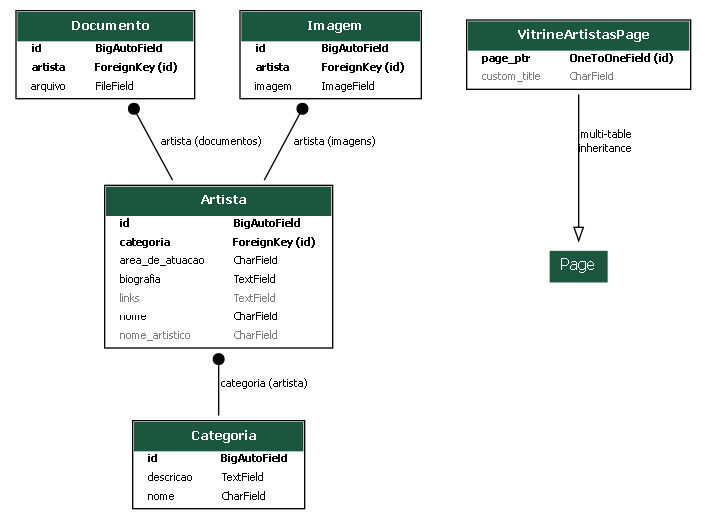
\includegraphics[scale=0.5]{./img/er_diagram_vitrine.png}
	   \legend{Fonte: Produzido pelo autor}
	 \end{minipage}
\end{figure}

\subsubsubsection{Escola de Artes}

O modelo de dados para a Escola de Artes é estruturado de forma a atender às diversas necessidades operacionais e acadêmicas da instituição. Este modelo é essencial para o gerenciamento eficaz dos cursos, alunos, responsáveis, professores, e outros aspectos relacionados ao bom funcionamento da escola.

A base do modelo é o Curso, que representa as disciplinas oferecidas pela escola. Cada curso é caracterizado pelo nome, disciplina, turno e número de vagas disponíveis. As disciplinas são limitadas a um conjunto fixo, incluindo opções como Capoeira, Violão e Pintura e Desenho. O turno do curso pode ser Manhã, Tarde ou Noite, e o número de vagas é validado para garantir que se mantenha dentro de um intervalo apropriado.

Os Responsáveis são os indivíduos que, muitas vezes, são os pais ou responsáveis legais dos alunos. Cada responsável possui informações detalhadas como nome, CPF, data de nascimento, e-mail, endereço e telefone. Além disso, o modelo inclui a capacidade de anexar documentos relevantes e gerar um link único para configurar o acesso ao sistema através do modelo User do Django, com uma relação de um-para-um. A associação de um responsável com um aluno é feita através do campo responsavel, permitindo múltiplos responsáveis para cada aluno, se necessário.

O modelo de Aluno captura informações abrangentes sobre os estudantes, incluindo nome, CPF, RG, data de nascimento, e-mail, endereço e telefone. Os alunos podem ter documentos anexados e, caso sejam dependentes, são vinculados a responsáveis através de uma relação de muitos-para-muitos. Cada aluno também possui um link único para configurar o acesso ao sistema através do modelo User do Django com uma relação de um-para-um, caso ele não seja um dependente.

Os Professores são representados com detalhes como nome, especialidade, e-mail e telefone. Eles são associados aos cursos através das turmas e têm uma relação de um-para-um com o modelo User do Django, permitindo o gerenciamento de suas credenciais de acesso.

As Turmas são associadas a um curso e a um professor, e podem ter vários alunos. Cada turma possui um nome e horário específicos, facilitando a organização das aulas e a alocação dos recursos.

O Diário de Classe é um registro diário das atividades da turma. Cada entrada no diário está associada a uma turma específica e a uma data, proporcionando uma visão detalhada do progresso e das atividades da turma ao longo do tempo. O data do diário é adicionada automaticamente de acordo com o dia atual no momento da criação do diário.

Para registrar ocorrências, acompanhar a frequência e a pontuação dos alunos, foram criados os modelos Ocorrência, Frequência e Pontuação. O modelo de Ocorrência documenta eventos específicos que afetam um aluno em um determinado dia, enquanto o modelo de Frequência rastreia a presença dos alunos e permite justificativas para ausências. A Pontuação avalia o desempenho dos alunos em diferentes aspectos, como assiduidade, comportamento e aptidão. Esses dados são críticos para monitorar o progresso dos alunos e identificar áreas que necessitam de atenção.

Finalmente, o modelo de Inscrição registra as inscrições dos alunos em cursos específicos, incluindo observações adicionais e a data de inscrição. Este modelo garante que o processo de matrícula seja registrado de maneira estruturada e eficiente. Abaixo está descrito com mais detalhes o diagrama ER da Escola de artes.


\begin{figure}[htb]
	\centering
	 \begin{minipage}{0.4\textwidth}
	   \centering
	   \caption{Diagrama ER da Escola de Artes} \label{er_diagram_escola}
	   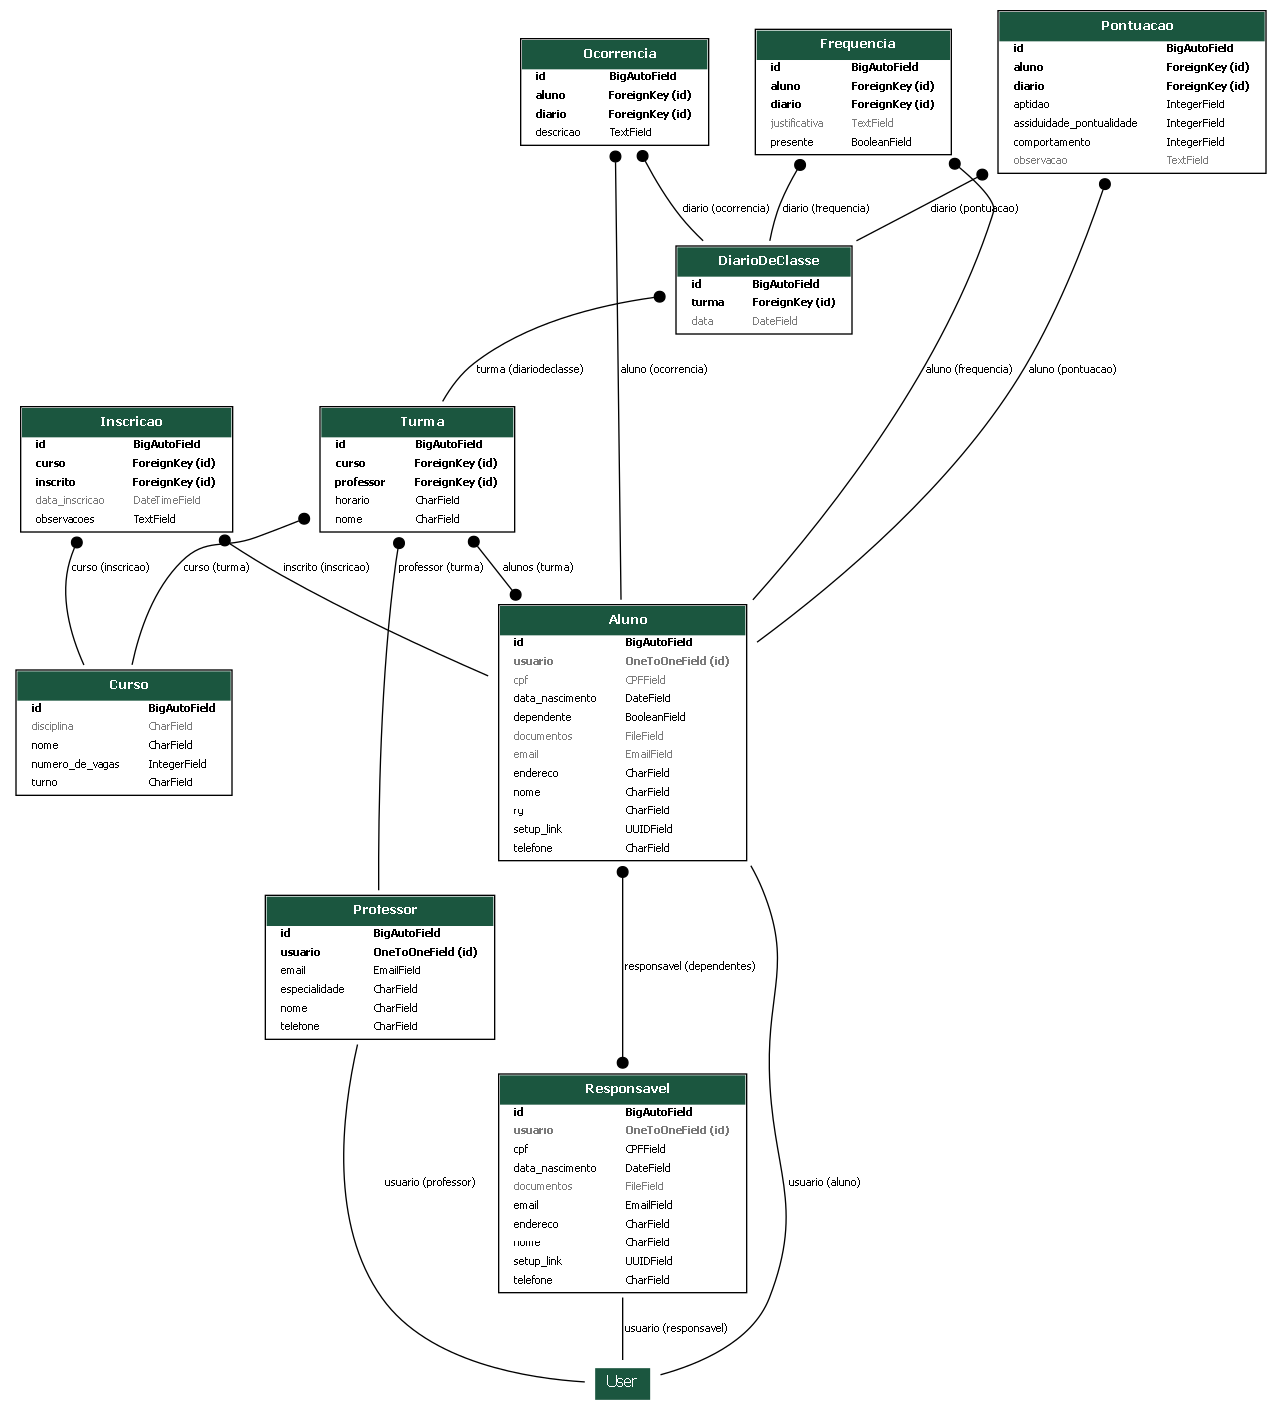
\includegraphics[scale=0.25]{./img/er_diagram_escola.png}
	   \legend{Fonte: Produzido pelo autor}
	 \end{minipage}
   \end{figure}

\subsubsubsection{Editais}

O modelo de dados para a seção de Editais é crucial para a gestão e operacionalização de processos seletivos e inscrições dentro do sistema. Este conjunto de modelos foi desenvolvido para facilitar a criação, gerenciamento e inscrição em editais, bem como para a comunicação eficiente com os participantes.

O Edital é a entidade fundamental do sistema, representando um processo seletivo ou oportunidade de inscrição. Cada edital possui um título, uma descrição detalhada, um período de inscrição definido por uma data e hora de início e término, e um status que pode ser "Aberto", "Fechado" ou "Indisponível". O status do edital é dinamicamente atualizado através do método "atualizar\_status", que compara a data e hora atuais com o período de inscrição para determinar se o edital está aberto para novas inscrições. Caso o edital esteja fora do período de inscrição, seu status é atualizado para "Fechado".

O modelo de Inscrição é utilizado para registrar as inscrições de candidatos em editais específicos. Cada inscrição está associada a um edital e contém informações do candidato, como nome, e-mail e um documento de apoio. Além disso, a inscrição inclui um campo de protocolo único, gerado com base no ID do edital, ID do usuário e ID da própria inscrição. Esse protocolo é atribuído no momento da criação da inscrição. O modelo também possui um campo para marcar a aprovação da inscrição e, se aprovado, um e-mail de chamamento é enviado ao candidato, informando-o sobre sua aprovação.

A classe EditaisPage é uma página do Wagtail que exibe uma lista de editais disponíveis. Esta página usa um template para apresentar a lista de editais e permite personalizar o título da página. O método get\_context é usado para adicionar todos os editais ao contexto da página, garantindo que a lista mais atualizada de editais esteja disponível para visualização.

Similarmente, a EditailInscreverPage é uma página do Wagtail dedicada aos detalhes de um edital específico, permitindo que os usuários visualizem informações detalhadas sobre o edital e se inscrevam. Esta página também utiliza um template e permite a personalização do título. O método get\_context é utilizado para fornecer o contexto necessário, incluindo todos os editais disponíveis.

Este conjunto de modelos fornece uma estrutura robusta para o gerenciamento de editais e inscrições, garantindo que as informações sejam mantidas de forma organizada e acessível. Além disso, as funcionalidades integradas de atualização de status e envio de e-mails ajudam a manter a comunicação fluida e eficiente com os participantes, enquanto as páginas do Wagtail oferecem uma interface amigável para a visualização e interação com os editais.

\begin{figure}[htb]
	\centering
	 \begin{minipage}{0.4\textwidth}
	   \centering
	   \caption{Diagrama ER dos Editais} \label{er_diagram_editais}
	   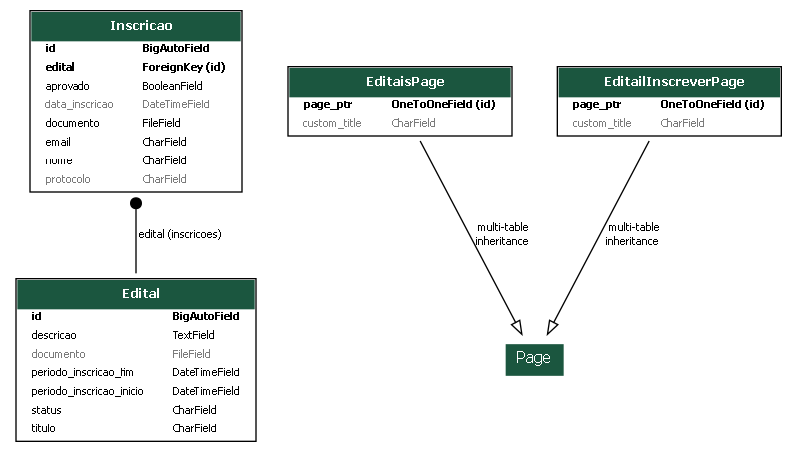
\includegraphics[scale=0.5]{./img/er_diagram_editais.png}
	   \legend{Fonte: Produzido pelo autor}
	 \end{minipage}
   \end{figure}


\subsubsection{Integração com o site}

\section{Organização do trabalho}

\textbf{É importante observar que a estrutura é apresentada a partir do próximo capítulo. O capítulo de Introdução não deve compor esta descrição. Além disso, sempre que você fizer referência à algum item específico, a inicial deve ser maiúscula. Por exemplo, Capítulo 2, Tabela 5, Figura 1, dentre outros.}

O restante deste trabalho é organizado como se segue. O Capítulo~\ref{cap:revisao} apresenta...
